\section{Background}

\subsection{Central Nervous System}

The core component of the nervous system in general, and the brain in particular, is the neuron. A neuron is an electrically excitable cell that processes and transmits information by electro-chemical signalling. The average human brain has about 100 billion neurons. Each neuron may be connected to up to $10,000$ other neurons, passing signals to each other via as many as $1,000$ trillion synaptic connections. \cite{brain}\par
The main function of the white matter is to connect neurons from different brain regions to each other by myelinated nerve fibers. \cite{white} The myelin sheath is a greatly extended and modified plasma membrane wrapped around the nerve axon in a spiral fashion. \cite{myelin}\par

\subsection{Magnetic Resonance Imaging}

\ac{DTI} is a noninvasive, quantitative \ac{MRI} technique that measures the rate and direction of movement of water molecules within tissues. In the \ac{CNS}, axonal tracts and myelin present physical barriers that impose directionality or anisotropy on water diffusion (\reflink{fig:dti}{Figure}). Applying magnetic field gradients allows the measurement of the rate and direction of the movement of water molecules in the direction of the magnetic field. Using the basis of diffusion, we can construct a 3D directional architecture of axon fibers and myelin in the \ac{CNS}. \cite{dti}
\begin{figure}[H]
\centering
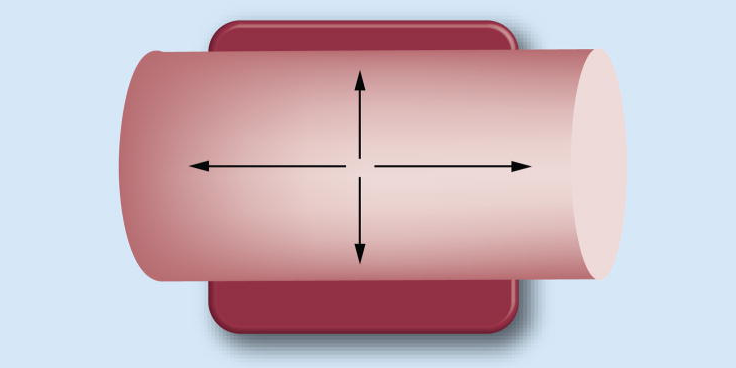
\includegraphics[width=0.4\textwidth]{dti0}
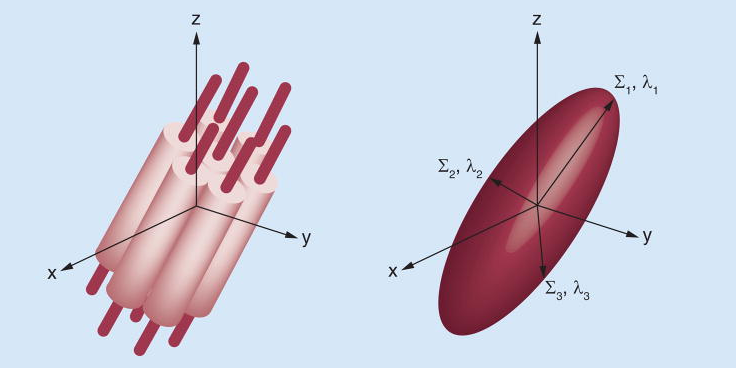
\includegraphics[width=0.4\textwidth]{dti1}
\caption{Physical Barrier Restricting Diffusion}
\label{fig:dti}
\end{figure}
However, due to \ac{DTI} is not being part of many clinical protocols, and it taking a relatively long time to acquire, it is not widely available in datasets. Other more basic \ac{MRI} methods, like the T1 and T2 weighted images are far more common, and part of many clinical protocols. These anatomical \ac{MRI} techniques are far more simple, and can mainly be used to differentiate between tissue types, without containing information about the fibers' directionality (like in \ac{DTI}).

\subsection{Radiomics}

Although the term is not strictly defined, radiomics generally aims to extract quantitative, and ideally reproducible, information from diagnostic images, including complex patterns that are difficult to recognize or quantify by the human eye. \cite{radio} Radiomic features can be extracted voxel and non-voxel based. Where in the prior case the features are extracted for each voxel, from around their vicinity, using a similar kernel based approach to convolution. Where in the non-voxel based approach the features are extracted for any arbitrary mask acting as a kernel (this could also mean the entire brain itself).\par
This feature extraction method can be invaluable when working with limited datasets, as a \ac{NN} based feature extraction such as a \ac{CNN} usually require vast amounts of training data.\par
Also some of these more complex radiomic features might be very challenging for a \ac{NN} to reproduce. For example the Gray Level Run Length Matrix Features describe the properties of extracted Gray Level Run Length Matrices from the image. Where said matrix quantifies gray level runs, which are defined as the length in number of pixels, of consecutive pixels that have the same gray level value. In a gray level run length matrix $P(i,j|\theta)$, the $(i,j)$ element describes the number of runs with gray level $i$ and length $j$ occur in the image along angle $\theta$. And an example of a feature could be the run length non-uniformity, measuring the similarity of run lengths throughout the image, with a lower value indicating more homogeneity among the run lengths. \cite{radio2}

\subsection{Basal Ganglia and Huntington’s Disease}

Basal ganglia is a part of the human brain which is a group of subcortical nuclei responsible primarily for motor control, as well as other roles such as motor learning, executive functions and behaviors, and emotions. \cite{basal} Huntington’s disease is a disorder that causes the progressive degeneration of the basal nuclei. \cite{hunting}\par

\section{State of the Art}

Certain images extracted from a \ac{DTI} record, like \ac{FA}, \ac{MD} and \ac{RD} are invaluable for characterizing, researching and diagnosing neurodegenerative diseases. Furthermore, a more complicated algorithm can be employed to extract information regarding the connectivity of brain regions, specifically using tractography methods to model the trajectories of white matter pathways. Tractography algorithms, such as probabilistic tractography, can simulate numerous potential pathways (tracts) originating from a seed region, or \ac{ROI} such as the Basal Ganglia.
\begin{figure}[H]
\centering
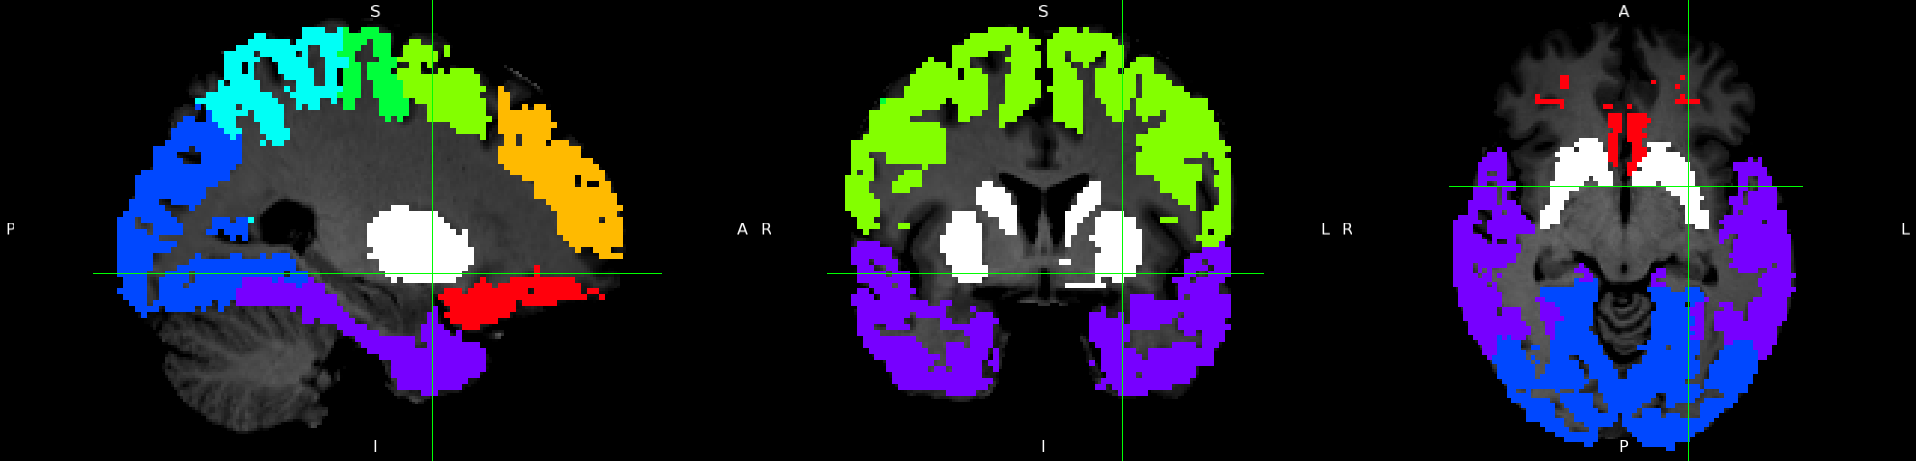
\includegraphics[width=1\textwidth]{rois}
\caption{Basal Ganglia (ROI) \& Cortical Targets}
\label{fig:rois}
\end{figure}
\begin{table}[H]
\centering
\begin{tabular}{|l|l|}
\hline
\textbf{Color} & \textbf{Region} \\ \hline
\begin{tikzpicture}\filldraw[draw=black,fill={rgb,255:red,255;green,255;blue,255}](0,0.15)rectangle(0.25,0.4);\end{tikzpicture} White & Basal Ganglia (ROI) \\ \hline

\begin{tikzpicture}\filldraw[draw=black,fill={rgb,255:red,255;green,0;blue,12}](0,0.15)rectangle(0.25,0.4);\end{tikzpicture} Red & Limbic \\ \hline

\begin{tikzpicture}\filldraw[draw=black,fill={rgb,255:red,255;green,186;blue,0}](0,0.15)rectangle(0.25,0.4);\end{tikzpicture} Orange & Executive \\ \hline

\begin{tikzpicture}\filldraw[draw=black,fill={rgb,255:red,131;green,255;blue,0}](0,0.15)rectangle(0.25,0.4);\end{tikzpicture} Light Green & Rostral-Motor \\ \hline

\begin{tikzpicture}\filldraw[draw=black,fill={rgb,255:red,0;green,255;blue,59}](0,0.15)rectangle(0.25,0.4);\end{tikzpicture} Green & Caudal-Motor \\ \hline

\begin{tikzpicture}\filldraw[draw=black,fill={rgb,255:red,0;green,255;blue,246}](0,0.15)rectangle(0.25,0.4);\end{tikzpicture} Light Blue & Parietal \\ \hline

\begin{tikzpicture}\filldraw[draw=black,fill={rgb,255:red,0;green,72;blue,255}](0,0.15)rectangle(0.25,0.4);\end{tikzpicture} Blue & Occipital \\ \hline

\begin{tikzpicture}\filldraw[draw=black,fill={rgb,255:red,119;green,0;blue,255}](0,0.15)rectangle(0.25,0.4);\end{tikzpicture} Purple & Temporal \\ \hline
\end{tabular}
\caption{Regions Legend}
\label{tab:reglen}
\end{table}
These tracts can be traced to determine their likelihood of reaching specific target regions, such as cortical areas of interest in \reflink{tab:reglen}{Table}. Each voxel within the seed region can be assigned a connectivity value based on the proportion of simulated tracts that successfully reach a given target region, providing a probabilistic measure of connectivity. Once these connectivity values are obtained, the seed region can be segmented, or parcellated, into distinct subregions that are preferentially connected to different targets. This connectivity based parcellation enables a detailed examination of the functional organization of brain regions and their relationship with target areas, contributing valuable insights into both healthy and pathological brain networks.
\begin{figure}[H]
\centering
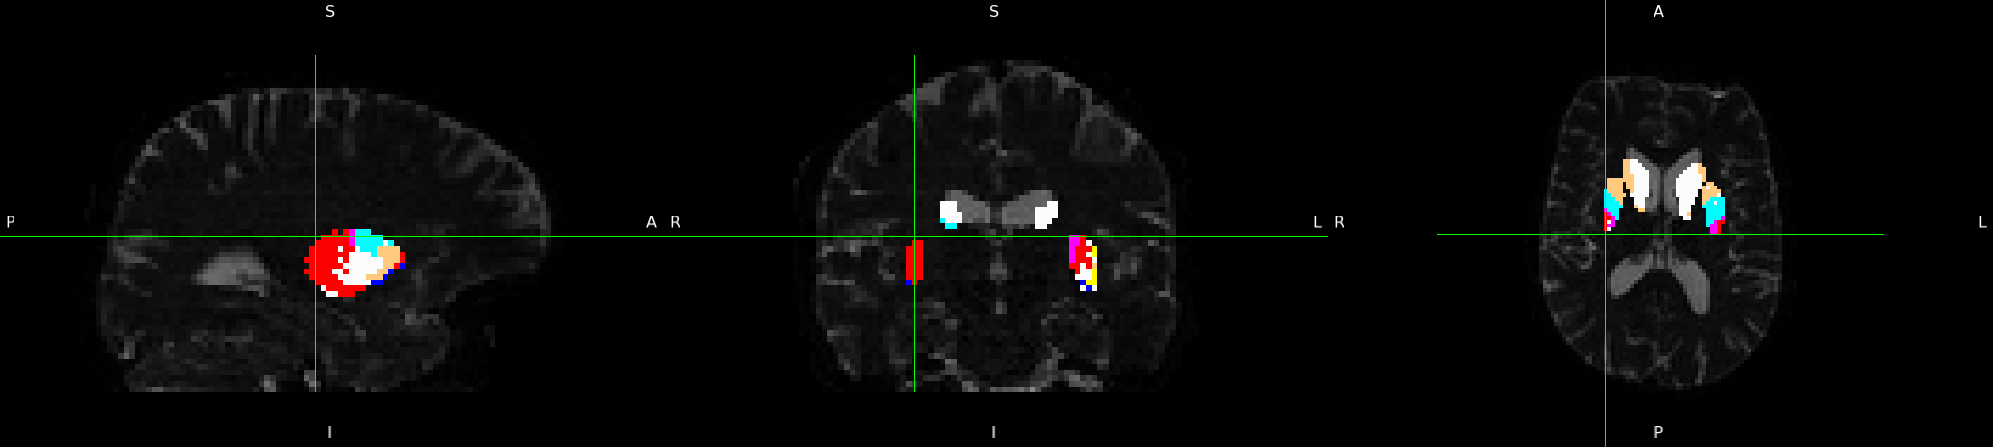
\includegraphics[width=1\textwidth]{conn}
\caption{Basal Ganglia Parcellation}
\label{fig:conn}
\end{figure}
Different studies have proposed that the ratio of the more commonly obtained T1 and T2 images, can serve as a proxy for myelin. \cite{myelin1} \cite{myelin2} Another study also investigated direct correlations between images \ac{MWF}, T1w/T2w ratio, \ac{FA}, \ac{RD} and \ac{MD}. \cite{myelin3}

\section{Motivation}

The recent studies mentioned in the previous section raise the question, what if some of these \ac{DTI} related images could be synthetized and predicted from simple structural T1 and T2 \ac{MRI} images. This would enable skipping the time and resource consuming process performing \ac{DTI} and potentially even further post processing algorithms like tractography. And it would also have the added benefit of being able to synthetize these less commonly available images from already available historical records.

\section{Objectives}

The goal of this research will be to try to predict \ac{FA} and \ac{MD} from the T1 and T2 images. With the additional goal of predicting relative connectivity. Furthermore, the experiments will include neurologically healthy participants (controls) and participants with Huntington's Disease (patients). This will allow making observations about the influence of neurodegeneration to the stability of the method.

\subsection{Delimitations}

This research will be limited to the Basal Ganglia as the \ac{ROI}, making it feasible for the timeframe of the thesis.

\subsection{Intermediate Goal}

A simpler, intermediate task leading up to the more complex end goals, is a model for the simple segmentation of the Basal Ganglia for the subcortical regions Caudate, Putamen and Accumbens. In order to confirm the feasibility of this project. This problem is inherently connected to the main goals, as the relative connectivity does obey certain anatomical restrictions, and the subcortical segmentation of the Basal Ganglia is confirmed to be related to the relative connectivity. Thus if this simpler prediction fails, it is almost certain that the complex end goals will fail as well.

\section{Previous Work}

\subsection{Participants}

In the clinical analysis, 47 patients with \ac{HD} were included, of which 24 of the gene mutation carriers were manifest (symptomatic) patients. And 23 of the gene mutation carriers were premanifest (asymptomatic) patients.\par
A total of 41 patients from the clinical analysis along with 32 healthy controls matched for age, sex, and years of education participated in the neuroimaging analysis. Out of which 22 patients were symptomatic, defined as those with a diagnostic confidence level of at least 4 on the \ac{cUHDRS}. And the rest 19 patients were asymptomatic participants. And three symptomatic patients did not undergo tractography analysis due to missing data.\par
None of the participants reported previous history of neurological disorder other than \ac{HD}. The study was approved by the ethics committee of Bellvitge Hospital in accordance with the Helsinki Declaration of 1975. All participants signed a written declaration of informed consent.

\subsection{Clinical Evaluation}

Three clinical domains (i.e. motor, cognitive, and behavioral) were evaluated using a battery of clinical scales and questionnaires. This included the \ac{cUHDRS}, which consists of motor, cognitive, and behavioral subscales \cite{uhdrs}.

\subsection{MRI Data Acquisition}
\ac{MRI} data were obtained using the 3T whole-body MRI scanner (Siemens Magnetom Trio; Hospital Clinic, Barcelona), with a 32-channel phased array head coil. Structural images included a conventional high resolution 3D T1 image, 208 sagittal slices, matrix 208×256×256, repetition time $1970$ms, echo time $2.34$ms, inversion time $1050$ms, flip angle $9^{\circ}$, field of view $256$mm, slice thickness $1$mm with no gap between slices.\par
Additionally, diffusion weighted \ac{MRI} was obtained. Diffusion weighted imaging was obtained using a diffusion tensor imaging sequence with a dual spin-echo \ac{DTI} diffusion imaging sequence with GRAPPA (reduction factor of $4$) cardiac gating, with echo time $92$ms, $2$mm isotropic voxels with no gap, $60$ axial slices, field of view $236$mm. To obtain the diffusion tensors, diffusion was measured along $64$ non-collinear directions, using a single b-value of $1500\frac{s}{mm^2}$ and interleaved with 9 non-diffusion $b=0$ images. Frequency selective fat saturation was used to suppress fat signal and avoid chemical shift artifacts.

\subsection{Tractography}
\ac{DTI} data were automatically processed using the \ac{FDT} in the \ac{FSL}. First, skull stripping was performed using the Brain Extraction Tool \cite{bet}. Head motion and eddy current correction were then applied, with the gradient matrix rotated accordingly \cite{eddy}.\par
A multi fibre diffusion model was fitted to the data using \ac{FDT} \cite{tract}, employing a Bayesian approach to estimate a probability distribution function for the principal fibre direction at each voxel, accommodating crossing fibres within each voxel \cite{tract2}.\par
In addition, affine intra subject non-linear transformation to an MNI152 template were calculated using \ac{FNIRT}, for both the diffusion weighted and the anatomical images. The diffusion tensor was reconstructed using a standard least squares tensor estimation algorithm for each voxel, and \ac{FA} and \ac{MD}, as an index of microstructural organisation map was calculated from corresponding eigenvalues and eigenvectors.

\subsection{Connectivity Calculation}

\subsubsection{Cortical Targets}
Cortical target regions were provided by \citelink{target}{Tziortzi} and consisted of Limbic, Executive, Rostral-Motor, Caudal-Motor, Parietal, Occipital and Temporal regions. All 7 regions were transformed from the normalized MNI152 T1 space to the participants’ native diffusion space via the \ac{FNIRT} warp fields.\par
The basal ganglia were segmented in the native T1 space into lateralised caudate, nucleus accumbens, and putamen using the FIRST toolbox in \ac{FSL}.\par
Following this, the segmented basal ganglia subcortical regions were warped to the participants’ native diffusion space following the same process as the cortical targets. The nucleus accumbens, caudate, and putamen were then combined to create \ac{ROI}s for each participant, to be used for connectivity based parcellation.

\subsubsection{Relative Connectivity}

Connectivity based hard parcellation of the basal ganglia was carried out using the "find the biggest" algorithm in \ac{FSL} \cite{biggest}, using the cortical classifiers. Specifically, the probtrackx2 function from the \ac{FDT} toolbox was employed using standard settings (number of streamlines $5000$, number of steps per sample $2000$, step length $0.5$mm, and curvature threshold $0.2$). All images were in the native diffusion space, with the seed as the basal ganglia and classification targets set as 14 cortical targets ($7$ targets x $2$ hemispheres, left and right) \cite{tract}. This resulted in the streamline image of the basal ganglia being segmented into 14 lateralised maps with regards their connectivity to each of the 7 cortical targets.\par
These connectivity based probabilistic streamline images had a set of values for each voxel of the basal ganglia which represents how many tractography samples out of the default setting of $5000$ reach the cortical targets. These images were then thresholded at $10$\% to remove noise and aberrant connections. Following this, relative connectivity maps were then calculated by dividing individual probabilistic images by the sum of all images, and then thresholding at $50$\% to minimize any overlap between these maps. These relative connectivity maps allowed for the measurement and comparison of changes in of topographically organized connectivity.

\subsection{Summary}

Hospital de Bellvitge provided an excellent dataset of anatomocal \ac{MRI} and \ac{DTI} records of 32 control and 38 \ac{HD} patient records of T1 and T1/T2 \ac{MRI} images with isotropic voxels of 1 millimeter resolution and \ac{DTI} \ac{FA} and \ac{MD} images with isotropic voxels of 2 millimeter resolution. Furthermore this dataset also contains the mask for the basal ganglia, which will also be referenced as the \ac{ROI}; masks for the 7 cortical regions of the brain, which will also be referenced as the target regions: Limbic, Executive, Rostral-Motor, Caudal-Motor, Parietal, Occipital and Temporal; streamline images and relative connectivity maps from the results of tractography; subcortical segmentation of the basal ganglia for the Caudate, Putamen and Accumbens; and \ac{FNIRT} warp fields for converting the records into normalized space.\par
Furthermore, for both the \ac{ROI} and cortical targets, the dataset distinguishes between the right and left hemispheres of the brain. Thus there are actually 2 \ac{ROI}s and $2 \cdot 7=14$ target regions.

